%Dokumenteinstellungen und Anpassungen
%Dokumentenklasse "scrbook" - Erweitert um den Verweis auf die Verzeichnisse und Texteigenschaften
\documentclass[12pt,a4paper,oneside,parskip=half,listof=totoc,bibliography=totoc,numbers=noendperiod,ngerman,dvipsnames]{scrartcl}
%Anpassung der Seitenränder (Standard bottom ca. 52mm anbzüglich von ca. 4mm für die nach oben rechts gewanderte Seitenzahl)
\usepackage[bottom=48mm,left=25mm,right=25mm]{geometry}

%Tweaks für scrbook
\usepackage{scrhack}

%Blindtext
%\usepackage{blindtext}

%Erlaubt unteranderem Umbrücke captions
\usepackage{caption}
\usepackage{derivative}
%Stichwortverzeichnis
\usepackage{imakeidx}
\usepackage{amsmath}
%Kompakte Listen
\usepackage{paralist}
% Multiline comments
\usepackage{comment}
%Zitate besser formatieren und darstellen
\usepackage{epigraph}
\usepackage{acronym}

%Glossar, Stichworverzeichnis (Akronyme werden als eigene Liste aufgeführt)
\usepackage[toc, acronym]{glossaries} 

%Anpassung von Kopf- und Fußzeile
%beinflusst die erste Seite des Kapitels
\usepackage[automark,headsepline]{scrlayer-scrpage}
%\automark{chapter}
\ihead{\leftmark}
\chead{}
\ohead{\thepage}
\ifoot*{}
\cfoot[\thepage]{}
\cfoot*{}
\ofoot*{\thepage}
\ofoot{Test}
\pagestyle{scrheadings}


%Auskommentieren für die Verkleinerung des vertikalen Abstandes eines neuen Kapitels
%\renewcommand*{\chapterheadstartvskip}{\vspace*{.25\baselineskip}}

%Zeilenabstand 1,5
\usepackage[onehalfspacing]{setspace}

%Verbesserte Darstellung der Buchstaben zueinander
\usepackage[stretch=10]{microtype}

%Deutsche Bezeichnungen für angezeigte Namen (z.B. Innhaltsverzeichnis etc.)
\usepackage[ngerman]{babel}

%Unterstützung von Umlauten und anderen Sonderzeichen (UTF-8)
\usepackage{lmodern}
\usepackage[utf8]{luainputenc}
\usepackage[T1]{fontenc}

%Einfachere Zitate
\usepackage{epigraph}

%Unterstützung der H positionierung (keine automatische Verschiebung eingefügter Elemente)
\usepackage{float} 

%Erlaubt Umbrüche innerhalb von Tabellen
\usepackage{tabularx}

%Erlaubt Seitenumbrüche innerhalb von Tabellen
\usepackage{longtable}

%Erlaubt die Darstellung von Sourcecode mit Highlighting
\usepackage{listings}

%Definierung eigener Farben bei nutzung eines selbst vergebene Namens
\usepackage[table,xcdraw]{xcolor}
\usepackage{pdfpages}
%Vektorgrafiken
\usepackage{tikz}

%Grafiken (wie jpg, png, etc.)
\usepackage{graphicx}

%Grafiken von Text umlaufen lassen
\usepackage{wrapfig}
\usepackage{pgfplots}

%Ermöglicht Verknüpfungen innerhalb des Dokumentes (e.g. for PDF), Links werden durch "hidelink" nicht explizit hervorgehoben
\usepackage[hidelinks,german]{hyperref}
\usepackage{cleveref}
\usepackage{siunitx}
\usepackage{physics}
\usepackage[most]{tcolorbox}
\newtcolorbox{mybox}{
	enhanced,
	boxrule=0pt,frame hidden,
	borderline west={4pt}{0pt}{green!75!black},
	colback=green!10!white,
	sharp corners
}
\newtcolorbox{qed}{
	enhanced,
	boxrule=0pt,frame hidden,
	borderline west={4pt}{0pt}{blue!75!black},
	colback=cyan!5!white,
	sharp corners
}
\usepackage{todonotes}
\usepackage{cancel}%Durchstreichen von sachen
\usepackage[numbered,framed]{matlab-prettifier}
%Einbindung und Verwaltung von Literaturverzeichnissen
\usepackage{csquotes} %wird von biber benötigt
\usepackage[style=ieee, backend=biber, bibencoding=ascii]{biblatex}
\addbibresource{references/references.bib}
\usepackage{multirow}
\usepackage{nicematrix}

\newenvironment{conditions}[1][mit:]
{#1 \begin{tabular}[t]{>{$}l<{$} @{${}={}$} l}}
	{\end{tabular}\\[\belowdisplayskip]}

\usepackage{fancyvrb}
\lstset{literate=% Allow for German characters in lstlistings.
	{Ö}{{\"O}}1
	{Ä}{{\"A}}1
	{Ü}{{\"U}}1
	{ß}{{\ss}}2
	{ü}{{\"u}}1
	{ä}{{\"a}}1
	{ö}{{\"o}}1
}
\usepackage{booktabs}
\usepackage{caption}
\usepackage{subcaption}

\definecolor{gray}{RGB}{127,127,127}
\definecolor{lightgray}{RGB}{219,219,219}
\definecolor{lightergray}{RGB}{237,237,237}

\DeclareSIUnit \voltampere {VA} %apparent power 
\DeclareSIUnit \VA {VA} %apparent power 
\DeclareSIUnit \var { var } %volt-ampere reactive - idle power 
%Anpassung der Überschriften
\addtokomafont{disposition}{\rmfamily}

%Zusätzliche Farben
\definecolor{darkgreen}{RGB}{0,100,0}

%Umbenennungen
\renewcommand{\lstlistlistingname}{Quelltextverzeichnis}

%Pluszeichen in der Referenc beim zitieren ausblenden
\renewcommand*{\labelalphaothers}{}

%Anpassugen zur Quelltextdarstellung, kann bei Bedarf überschrieben werden (z.B. wenn unterschiedliche Sprachen zum Einsatz kommen)
\renewcommand{\lstlistingname}{Codeauszug}
\lstset{
	language=Java,
	numbers=left,
	columns=fullflexible,
	aboveskip=5pt,
	belowskip=10pt,
	basicstyle=\small\ttfamily,
	backgroundcolor=\color{black!5},
	commentstyle=\color{darkgreen},
	keywordstyle=\color{blue},
	stringstyle=\color{gray},
	showspaces=false,
	showstringspaces=false,
	showtabs=false,
	xleftmargin=16pt,
	xrightmargin=0pt,
	framesep=5pt,
	framerule=3pt,
	frame=leftline,
	rulecolor=\color{green},
	tabsize=2,
	breaklines=true,
	breakatwhitespace=true,
	prebreak={\mbox{$\hookleftarrow$}}
}

%Anpassungen für das Abkürzungsverzeichnis
\newglossarystyle{dottedlocations}{%
	\renewcommand*{\glossaryentryfield}[5]{%
		\item[\glsentryitem{##1}\glstarget{##1}{##2}] \emph{##3}%
		\unskip\leaders\hbox to 2.9mm{\hss.}\hfill##5}%
	\renewcommand*{\glsgroupskip}{}%
}

%Titelformen - gewünschtes Layout einkommentieren

%%Graduation
\makeatletter

\newcommand*{\firstExaminer}[1]{\gdef\@firstExaminer{#1}}
\newcommand*{\subTitle}[1]{\gdef\@subTitle{#1}}
\newcommand*{\researchPart}[1]{\gdef\@researchPart{#1}}
\newcommand*{\matrikelnr}[1]{\gdef\@matrikelnr{#1}}
\newcommand*{\submitDate}[1]{\gdef\@submitDate{#1}}


\renewcommand*{\maketitle}{
	\begin{titlepage}
		\newgeometry{left=2.5cm,right=2.5cm,top=9.0cm,bottom=2.5cm}
		\begin{center}
			\vfill
			{\Large \@title\par}
			{\normalsize \@subTitle\par}
			\vskip 0.5cm
			{\large \bfseries Forschungsprojekt Teil \@researchPart\par}
			\vskip 0.5cm
			{\large an der}
			\vskip 0.5cm
			{\large Hochschule für Technik und Wirtschaft Berlin\\ Fachbereich Wirtschaftswissenschaften II\\ Studiengang Angewandte Informatik}
			\vfill
			\begin{flushleft}
				\begin{tabular}[t]{rl}
					Betreuer: &\@firstExaminer\\
					\\
					Eingereicht von: &\@author\\
					Matrikelnummer: & \@matrikelnr\\
					Datum der Abgabe: & \@submitDate
				\end{tabular}
			\end{flushleft}
		\end{center}
		\restoregeometry
	\end{titlepage}
}
\makeatother
%\gradeType{Angewandte Mathematik}
%\secondExaminer{Max Mustermann}

%Research paper
\include{titles/research_papger}
\subTitle{Leistungsöltransformator 50 Hz\\Leistungsstromrichter 16,7 Hz\\ 4QS Umrichter}
\researchPart{Bahnumricheranlage}

%Angaben zur Arbeit und dem Author (von beiden Layouts genutzt)
\title{Bahnumrichteranlage für 16.7 Hz und DC Zwischenkreis }
\author{Milan Daniel Larsen 581929}
\matrikelnr{581929}
\submitDate{30.06.2022}
\firstExaminer{Prof. Dr. S. Krämer}

%Verzeichnisse generieren
\makeglossaries
\loadglsentries{references/glossary_acronyms.tex}
\setacronymstyle{long-short}

\makeindex[columns=2, title=Stichwortverzeichnis, options= -s resources/styles/indexstyle.ist, intoc]
\indexsetup{level=\chapter*,toclevel=chapter}

%Start des Inhalts
\begin{document}

%Notwendiger Workaround
\pagenumbering{alph}

%Deckblatt erzeugen
\maketitle

\pagenumbering{Roman}

%\include{chapter/Vorwort} \clearpage
%\chapter*{Abstract}

\blindtext \clearpage

%Inhaltsverzeichnis
\tableofcontents \newpage

%Hauptteil
\pagenumbering{arabic}
% Allgemeine Einleitung und Erklärung
\section{Anlagenkonzept}
\subsection{Vergleich: TCR vs Statcom }
\section{Stromlaufplan}
\subsection{ Single-Line-Diagramm: Dynamischer Kompensationsanlage}
\section{Auslegung}
\subsection{Berechnungen}
\subsection{Filterkreiskondensator}  
\subsection{Filterkreisdrossel}
\subsection{Thyristorgesteuerte Drossel}
\subsection{Leistungsschalter}
\section{Detailbeschreibung}
\subsection{Erläuterungsbericht Auslegungsberechnungen}
\subsection{TCR-Regelstrategie}

\section{Literatur}
\subsection{SIEMENS 3AH3 Katalog} \clearpage
\section{Konzeptvergleich: Bahnumrichteranlagen}

Für eine Umrichteranlage zur Versorgung des Bahnstromnetzes aus dem Drehstromnetzt, können verschiedenen Konzepte zum Einsatz kommen.
Im Folgendem sollen diese Konzepte aus technischer und komerzieller Sicht Verglichen werden.

Es soll hier auf zwei Prinzipien eingegangen werden:

\textcolor{blue}{\textbf{Rotierender Umformer:}}
\\
Bei rotierenden Umformern werden in der Regel auf der Drehstromseite eine Dreiphasen-Asycnchronmaschiene mit der dreifachen Polzahl gegenüber der Einphasen-Synchronmaschiene auf der Bahnetzseite verwendet.

\textcolor{blue}{\textbf{Stationäre Umrichter:}}

Bei stationären Umrichtern kommt Halbleitertechnik zum Einsatz, um die benötigten Spannungen zu erzeugen. Bei indirekten Umrichtern wird, bei einem Energifluss ins Bahnnetz, mit einer Gleichrichter-Zwischenkreis-Wechselrichter
Topologie gearbeitet. 

\textcolor{blue}{\textbf{Vergleich der Konzepte:}}

\begin{tabular}{ l|l  }
   
    Rotierender Umformer & Stationäre Umrichter \\
    \hline
    \textbullet  \textcolor{red}{Komplexes bauliches Projekt (rotierende Massen)} & \textbullet  \textcolor{ForestGreen}{Einfacher Aufbau z.B. Container}\\
    \textbullet  \textcolor{red}{Hoher Wartungsaufwand (bemannt)} & \textbullet \textcolor{ForestGreen}{Geringer Wartungsaufwand} \\
    \textbullet \textcolor{ForestGreen}{Verfügbarkeit $\approx 93\%$} & \textbullet \textcolor{ForestGreen}{Verfügbarkeit $\approx 98\%$} \\ 
    \textbullet \textcolor{red}{Wirkungsgrad $\approx 92\%..95\%$} & \textbullet \textcolor{ForestGreen}{ Wirkungsgrad $\approx 97.5\%$  }\\
    \textbullet \textcolor{red}{ Dynamik begrenzt (rotierende Massen) $\approx \SI{10}{\MW\per\second}$}& \textbullet \textcolor{ForestGreen} {Hohe Dynamik $<\SI{500}{\MW\per\second}$} \\
    \textbullet \textcolor{ForestGreen}{Überlastbar (Netzstabilisierend)} & \textbullet \textcolor{red}{Geringe Überlastbarkeit }\\
    \textbullet \textcolor{ForestGreen}{4-Facher Kurschlussstrom }& \textbullet \textcolor{red}{$1.3$-Facher Kurzschlussstrom }\\
\end{tabular}


Der Stationäre Umrichter biete gegenüber dem rotierenden Umformer viele technische sowie monetäre Vorteile. 
Besonders der wartungsarm Betrieb und der bessere Wirkungsgrad wirken sich auf die laufenden Kosten aus.
Bei einem unterschied von $\Delta\eta\approx 5\%$ und einer Nennleistung von $P=\SI[]{17.5}{MW}$ hat der rotierende Umformer 
eine zusätzlichen Verlust von $\Delta P=\SI[]{875}{\kilo\watt}$. 
In einem Jahr Betrieb fallen damit $W=\SI{7.665}{\giga\watt\hour}$ zusätzliche Verlsutleistung an.

 \clearpage
\section{Drehstrom-Leistungstransformator 50 Hz}
Der Transformator soll für die Außenaufstellung ausgelegt werden und wird von 3 AC \SI[]{50}[]{\Hz}, \SI[]{110}[]{\kilo\volt} gespeist.
Der Transformator soll ölgefüllt und selbstkühlend sein.\\ 



\subsection{Allgemeine Merkmale}

\begin{table}[htb]
    \centering
    \begin{NiceTabular}{|l|c|}[]
        \CodeBefore
        \columncolor{lightergray}{1}
        \Body
        \hline
         Aufstellung & Freiluftaufstellung\\
         \hline
         Verschmutzung & Verschmutzungsgrad III (stark) \\
         \hline
         Aufstellungshöhe & < 1000 m üNN\\
         \hline
         Umgebungstemperatur &  -30°C bis 40°C\\
         \hline
         Klimabedingungen & Normal\\ 
         \hline
                 \Block{3-1}{Dokumentationen} &  \tabitem Technische Zeichnungen und CAD\\
                         &\tabitem Montageplan, Wartungsplan, Dokumentationen\\
                         &\tabitem Prüfprotokoll der zu erfüllenden Prüfungen\\
                         \hline
       
    \end{NiceTabular}
\end{table}

\pagebreak
\subsubsection*{Normen}

\begin{itemize}[noitemsep]
    \item DIN VDE 0532-76-1: Leistungstransformatoren\cite*{DINEN600761.}
    \item DIN EN 60076-3 Leistungstransformatoren Teil 3: Isolationspegel, Spannungsprüfungen und äußere Abstände in Luft \cite*{DINEN600763VDE0532763:201903.}
    \item DIN 60076-4 Leistungstransformatoren Teil 4: Leitfaden zur Blitz- und Schaltstoßspannungsprüfung von Leistungs-
    transformatoren und Drosselspulen\cite*{DINEN600764.2003}
    \item DIN 60076-10 Leistungstransformatoren Teil 10: Bestimmung der Geräuschpegel\cite*{DINEN600761.2002}
    \item DIN EN 60071-1 Isolationskoordination Teil 1: Begriffe, Grundsätze und Anforderungen\cite*{DINEN600711.2010}
\end{itemize} 

\subsubsection*{Schaltbild}
\begin{figure}[htb]
\centering
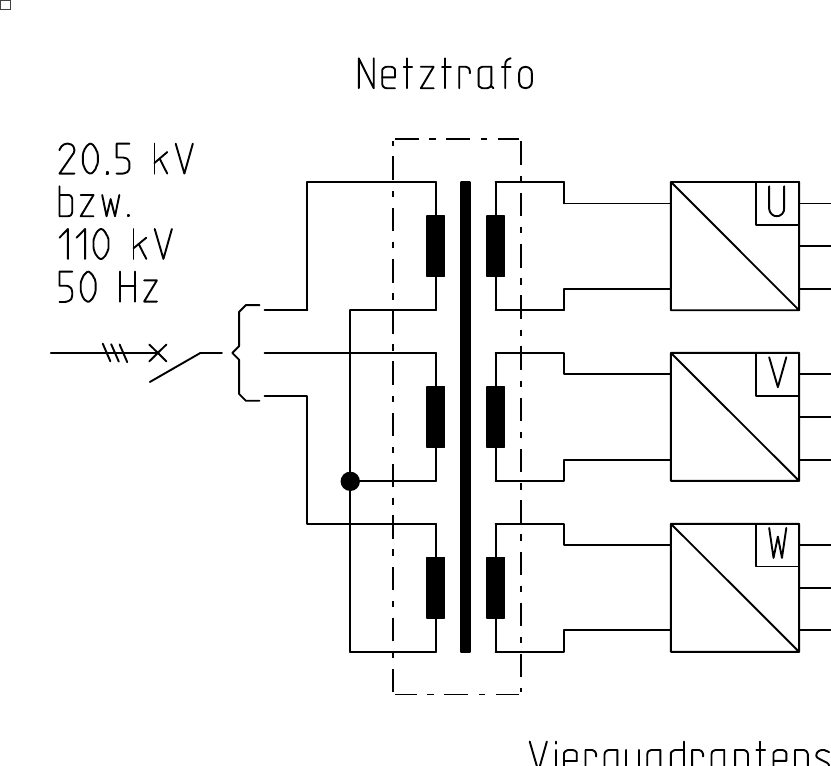
\includegraphics[width=\textwidth/2,frame]{Bilder/netztrafo.png}
\end{figure}
\subsection{Bemessungsdaten:}

\begin{table}[htb]
    \centering
    \begin{NiceTabular}{|l|p{2cm}|p{2cm}|}[hvlines]
        \CodeBefore
        \columncolor{lightergray}{1}
        \Body
       \Block{2-1}{Schaltgruppe} & OS & US \\ 
                                & Y(N) &   i0i0i0  \\
         Nennleistung ohne Leistung der Filterwicklung & \Block{1-2}{$\SI{17.68}{\unit{\mega\volt\ampere}}$}\\
         Nennspannung OS (Klemmenspannung) & \Block{1-2}{$\SI{110}{\kV}$}\\
         Max. Spannung OS (Klemmenspannung) & \Block{1-2}{$\SI{123}{\kV}$}\\
         Nennspannung US (Klemmenspannung) & \Block{1-2}{$\SI{3536}{\V}$}\\
         Nennstrom der US bei Nennspannung & \Block{1-2}{$\SI{1.667}{\kilo\ampere}$}\\
    \end{NiceTabular}
\end{table}

\textbf{Relative Kurzschlussspannungen:}
\begin{itemize}
    \item Bezugsgrößen: \\ bezogen auf Nennleistung bei $\SI{75}{\degree}$C; eine US Wicklung kurzgeschlossen; alle anderen Wicklungen offen; Speisung in OS Wicklung
    \item Werte \\ $uk_\mathrm{OS_iUS_i}\mathrm{(mit\,i=1...3)}=20\% (20.9\%...23.1\%)$; bezogen auf Nennleistung\\ $uk_\mathrm{US-US}>22\%$ (für alle Paarungen)
\end{itemize}

\subsubsection*{Verluste}
\begin{table}[htb]
    \centering
    \begin{NiceTabular}{|l|c|c|}[hvlines]
        \CodeBefore
        \columncolor{lightergray}{1}
        \Body
        &Grundschwingung&Umrichterbetrieb (Zusatzverluste)\\
        Leerlaufverluste bei Nennspannung &  tbd. kW&<1\% von der Grundschwingung\\
        Kurzschlußverluste bei 75 °C &tbd. kW&<1\% von der Grundschwingung\\
    \end{NiceTabular}
\end{table}
\clearpage

\subsubsection*{Stromwandler}

\begin{table}[!htb]
    \centering
    \begin{NiceTabular}{|l|c|}[hvlines]
        \CodeBefore
        \columncolor{lightergray}{1}
        \Body
        \Block{2-1}{Stromwandler OS-Seite} &  3xtbd/1A; 15VA; 10P10\\
                                & 3xtbd/1A; 15VA; 0,5 FS10\\
                                Stromwandler US-Seite &3x tbd/1A;15VA;10P10\\
                                Stromwandler Kesselschutz &1x 100/1A;3VA;5P20\\
    \end{NiceTabular}
\end{table}

\subsubsection*{Durchführungen}
\begin{table}[h]
    \centering
    \begin{NiceTabular}{|l|c|}[hvlines]
        \CodeBefore
        \columncolor{lightergray}{1}
        \Body
        OS& 3 (+1 optional Sternpunkt herausführbar)\\
        US & 3x2 \\
    \end{NiceTabular}
\end{table}

\textbf{Isolation (nach Prüfungsnorm in \cite*{DINEN600763VDE0532763:201903.}):}
\begin{table} [h]
    \centering
    \begin{NiceTabular}{|l|c|c|}[hvlines]
        \CodeBefore 
        \columncolor{lightergray}{1}
        \Body
             & OS & US gegen Erde \\ 
           max. Betriebsspannung  & $\SI{123}{\kilo\volt}$ &  $\SI{7.2}{\kilo\volt}$ \\
         Nennstehwechselspannung & $U_1=$\SI{185}{\kilo\volt}; $U_2=$\SI{230}{\kilo\volt}& \SI{20}{\kilo\volt} \\
         Nennstehblitzspannung & $U_1=$\SI{450}{\kilo\volt}; $U_2=$\SI{550}{\kilo\volt}&$U_1=$\SI{40}{\kilo\volt}; $U_2=$\SI{60}{\kilo\volt}\\
    \end{NiceTabular}
\end{table}

\subsubsection*{Sternpunktausführung}
Der Sternpunkt OS ist aus der Wicklung herauszuführen und eine spätere Verwendung vorzubereiten. Durchführung und Isolator sind nicht erforderlich, der Sternpunkt kann blind verflanscht werden. 

\textbf{Kapazitive Kopplung}\\
Eine kapazitive Übertragung von Blitzüberspannungen von der OS-Wicklung auf die US-Wicklung ist zu vermeiden. Bisherige Transformatoren in Bahnkupplungen hatten zu diesem Zweck Schirmwicklungen. 
 
\textbf{Geräuschpegel}\\
Aufstellungsort: Allgemeines Wohngebiet gemäß § 1 BImSchG  $L_\mathrm{pmax}=40 dB(A)$.
Grenzwert darf im Fernfeld(5m) mit Messung nach DIN EN 60076-10 nicht überschritten werden.
 \clearpage
\section{Einphasen-Stromrichteröltrafo 16.7 Hz}
Der \SI[]{16.7}[]{\Hz} Transformator ist ein Summiertransformator und addiert die
Teilspannungen der Umrichter auf die Bahnspannung 2 AC
\SI[]{110}[]{\kV}. Der Transformator ist ölgefüllt, selbstkühlend und für die Aussenaufstellung ausgelegt.

\subsection{Allgemeine Merkmale}

\begin{table}[htb]
    \centering
    \begin{NiceTabular}{|l|c|}[]
        \CodeBefore
        \columncolor{lightergray}{1}
        \Body
        \hline
         Aufstellung & Freiluftaufstellung\\
         \hline
         Verschmutzung & Verschmutzungsgrad III (stark) \\
         \hline
         Aufstellungshöhe & < 1000 m üNN\\
         \hline
         Umgebungstemperatur &  -30°C bis 40°C\\
         \hline
         Klimabedingungen & Normal\\ 
         \hline
                 \Block{3-1}{Dokumentationen} &  \tabitem Technische Zeichnungen und CAD\\
                         &\tabitem Montageplan, Wartungsplan, Dokumentationen\\
                         &\tabitem Prüfprotokoll der zu erfüllenden Prüfungen\\
            \hline
    \end{NiceTabular}
\end{table}

\subsubsection*{Normen}
\begin{itemize}[noitemsep]
    \item DIN VDE 0532-76-1: Leistungstransformatoren
    \item DIN EN 61378-1 Stromrichtertransformatoren - Teil 1: Transformatoren für industrielle Anwendungen
    \item DIN EN 60076-3 Leistungstransformatoren Teil 3: Isolationspegel, Spannungsprüfungen und äußere Abstände in Luft
\end{itemize}
\subsubsection*{Schaltbild}
\begin{figure}[htb]
\centering
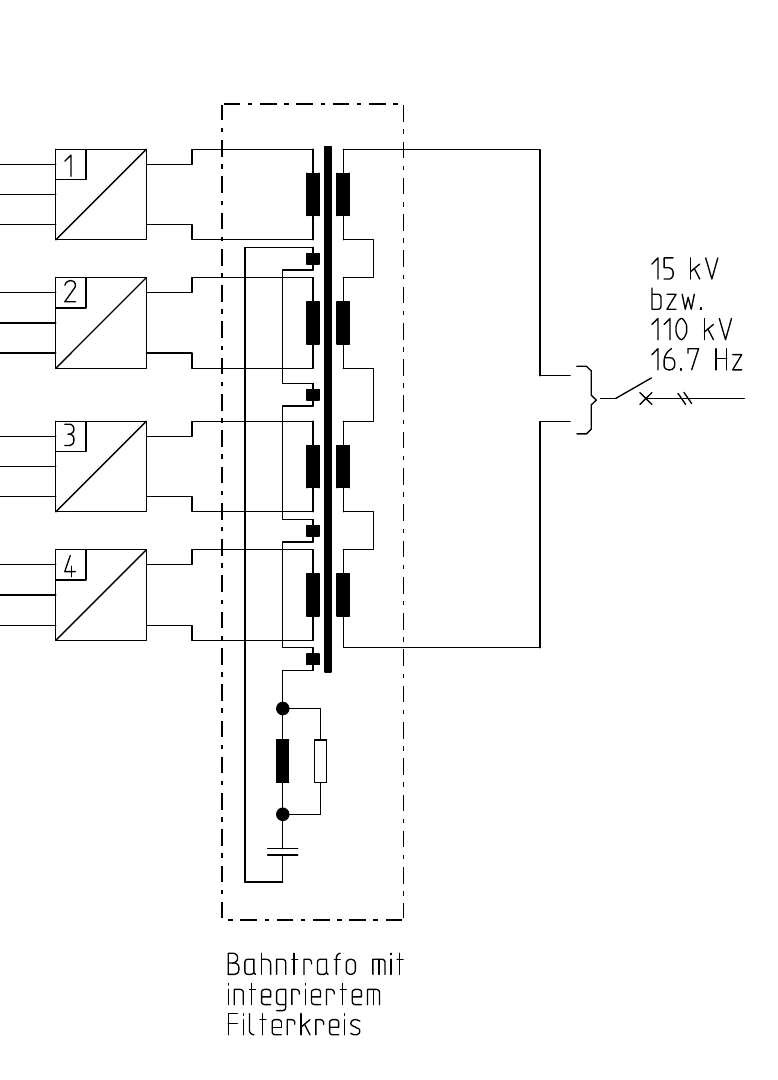
\includegraphics[width=\textwidth/3,frame]{Bilder/stromrichtertrafo.png}
\end{figure}
\clearpage
\subsection{Bemessungsdaten:}
\begin{table}[htb]
    \centering
    \begin{NiceTabular}{|l|p{2cm}|p{2cm}|}[hvlines]
        \CodeBefore
        \columncolor{lightergray}{1}
        \Body
       \Block{2-1}{Schaltgruppe} & OS & US \\ 
                                & | &   i0i0i0  \\
         Nennleistung ohne Leistung der Filterwicklung & \Block{1-2}{$\SI{20}{\unit{\mega\volt\ampere}}$}\\
         Leistung US Wicklung & \Block{1-2}{$4\cdot\SI{5.125}{\mega\VA}$}\\
         Nennfrequenz nach DIN EN 50163/A1 \cite{DeutschesInstitutfurNormungene.V..200802} & \Block{1-2}{$\SI{16.7}{\Hz}-6\%+4\%$}\\
         Nennspannung der OS-Wicklung  & \Block{1-2}{$\SI{110}{\kilo\V}$}\\
         Nennspannung einer US Wicklung bei \SI[]{110}[]{\kV} & \Block{1-2}{$4\cdot\SI{3535}{\kV}$}\\
         Nennstrom US-Wicklung bei Nennspannung & \Block{1-2}{$\SI{1414}{\A}$}\\
        Filterwicklung (HW) Nennleistung & \Block{1-2}{$\SI{4.8}{\mega\VA}$}\\
        Filterwicklung (HW) Nennspannung & \Block{1-2}{$\SI{6}{\kilo\V}$}\\
    \end{NiceTabular}
\end{table}

\subsubsection{Kurzschlussspannung, Impedanzen}
\tabitem 112 MVA; 110kV, beide US-Wicklungen kurzgeschlossen \ang{75}C
\begin{table}[htb]
    \centering
    \begin{NiceTabular}{|l|c|}[hvlines]
        \CodeBefore
        \columncolor{lightergray}{1}
        \Body
        OS-HW& $15\pm \SI[]{5}[]{\percent}(\SI[]{14.225}{\percent}...\SI[]{15.75}[]{\percent})$\\   
        US-HW& $\SI[]{9.4}[]{\percent}$\\
        US-HW& $\SI[]{5.6}[]{\percent}$\\
    \end{NiceTabular}
\end{table}

\subsubsection*{Verluste}
\begin{table}[h]
    \centering
    \begin{NiceTabular}{|p{5cm}|c|c|}[hvlines]
        \CodeBefore
        \columncolor{lightergray}{1}
        \Body
       &Grudnschwingung&Umrichterbetrieb(Zusatzverluste)\\
       Leerlaufverluste bei Nennspannung&tbd. \unit{\kW}& < \SI[]{1}[]{\percent} von der Grudnschwingung\\
    Kurzschlussverluste bei \ang{75}C&tbd. \unit{\kW}&< \SI[]{1}[]{\percent} von der Grudnschwingung\\
    \end{NiceTabular}
\end{table}

\subsubsection*{Isolation}
Die Blitzstoß- so wie die angelegte Stehwechselspannungsprüfung (ACSD)  muss als Stückprüung nach DIN EN 60076-3\cite*{DINEN600763VDE0532763:201903.} für alle Wicklungen des Transformators durchgeführt werden.
\begin{table}[htb]
    \centering
    \begin{NiceTabular}{|p{5cm}|c|c|c|}[]
        \CodeBefore
        \columncolor{lightergray}{1}
        \Body
        \hline
        &OS&US&FW\\
        \hline
       max. Betriebsspannung Leiter gegen Erde  &  \SI{123}{\kilo\V} & \SI{17.5}{\kilo\V} & \SI{7.2}{\kilo\V}\\
       \hline
       Nennstehwechselspannung gegen Erde & $U_1=$\SI{185}{\kilo\volt}; $U_2=$\SI{230}{\kilo\volt} & \SI{38}{\kilo\V} & \SI{20}{\kilo\V}\\
        \hline  
     \Block{2-1}{Nennstehblitzspannung} &$U_1=$\SI{550}{\kilo\volt}&$U_1=$\SI{95}{\kilo\volt}&$U_1=$\SI{60}{\kilo\volt}\\
        & $U_2=$\SI{450}{\kilo\volt}& $U_2=$\SI{75}{\kilo\volt}&$U_2=$\SI{40}{\kilo\volt}\\
        \bottomrule
    \end{NiceTabular}
\end{table}
\subsubsection*{Kapazitive Kopplung}
Eine kapazitive Übertragung von Blitzüberspannungen von der OS-Wicklung auf die US-Wicklung ist zu vermeiden. Bisherige Transformatoren in Bahnkupplungen hatten zu diesem Zweck Schirmwicklungen. 
 
\subsubsection*{Anschlüsse}

\begin{table}[htb]
    \centering
    \begin{NiceTabular}{|l|cccc|}[]
        \CodeBefore
        \columncolor{lightergray}{1}
        \Body
        \hline
        &&OS&US&FW\\
        \hline
            Anzahl der Durchführungen & Klemme&2&4x2&2\\
        \hline
        Art der Durchführung & Klemme & Porzellan & Porzellan & Porzellan\\
        \hline
    \end{NiceTabular}
\end{table}
Anschlusskabel Filter in einem Klemmkasten; 1 Kabel á  \SI{50}{\mm\squared} je  Anschluss  Filterwicklung

\subsubsection*{Stromwandler}

\begin{table}[htb]
    \centering
    \begin{NiceTabular}{|l|c|}[hvlines]
        \CodeBefore
        \columncolor{lightergray}{1}
        \Body
        \hline
        4 Stromwandler  sekundärseitig & tbd/1A;15VA; 10P10 \\
        1 Stromwandler  Filterseitig & tbd/1A;  15VA; 10P10 \\
        1 Stromwandler primärseitig & tbd/1A;  15VA; 10P10 \\
        1 Stromwandler Kesselschutz & tbd/1A;    3VA;  5P20 \\
    \end{NiceTabular}
\end{table}

\subsubsection*{Kessel}
 \clearpage
\section{Anforderungen an 50Hz und 16,7 Hz-Transformatoren}

\subsubsection*{ALlgemiene Technische Anforderungen}
\begin{table}[htb]
    \centering
    \begin{NiceTabular}{|l|p{8cm}|}[]
        \CodeBefore
        \columncolor{lightergray}{1}
        \Body
        \hline
         Aufstellung & Freiluftaufstellung\\
         \hline
         Verschmutzung & Verschmutzungsgrad III (stark) \\
         \hline
         Aufstellungshöhe & < 1000 m üNN\\
         \hline
         Umgebungstemperatur &  -30°C bis 40°C\\
         \hline
         Klimabedingungen & Normal gem. VDE 0532(IEC76-1)für Freiluftaufstellung\\ 
         \hline
                 \Block{3-1}{Dokumentationen} &  \tabitem Technische Zeichnungen und CAD\\
                         &\tabitem Montageplan, Wartungsplan, Dokumentationen\\
                         &\tabitem Prüfprotokoll der zu erfüllenden Prüfungen\\
                         \hline
                         maximale Kühlmitteltemperatur &  \ang{40}C\\
                         \hline
                         mittl. Wicklungsübertemperatur & \SI{65}{\kelvin} bei Nennleistung\\
                         \hline
                         Übertemperatur Öl oben & \SI{60}{\kelvin}\\
            \hline
            Schalldruckpegel Mittelwert; in 1m Abstand
    \end{NiceTabular}
\end{table}

\subsubsection*{Kühlung}

Kühlung: ONAN; 
ONAF vorbereitet (an den Kühlern wird eine Halterung vorgesehen, an der geeignete Lüfter installiert werden können; keine Leistungssteigerung)
\begin{table}[htb]
    \centering
    \begin{NiceTabular}{|l|c|p{5cm}|}
        \CodeBefore
        \columncolor{lightergray}{1}
        \Body
        \hline
        Kühlungsvariante &Innerer Kühlkreislauf &Äußerer Kühlkreislauf \\
        \hline
            ONAN& natürliche Konvektion Öl (Oil Natural)& natürliche Konvektion Umgebungsluft und Wärmestrahlung der Oberfläche (Air Natural)\\
            \hline
            ONAF& natürliche Konvektion Öl (Oil Natural)& erzwungene Konvektion Umgebungsluft und Wärmestrahlung der Oberfläche (Air Forced) \\
            \hline
    \end{NiceTabular}
\end{table}
\subsubsection*{Blechqualität}
durch Hersteller festzulegen
\subsubsection*{Induktion}
bei Nennleerlaufspannung:	$B=\SI[]{1.6}[]{\tesla}$\\
Sättigungskennlinie ist zu liefern

\subsubsection*{Halterungen für eine Traverse für die Kabel zum Umrichter}
Am Transformatorkessel soll  eine Traverse montiert werden, auf der die Kabel zum Umrichter verlegt werden.

\subsubsection*{Angaben zur Betriebsweisen}
\begin{itemize}
    \item Beide Transformatoren werden im gesamten Bereich $cos(\phi)=0.8\ldots-0.8$ betrieben. Die Transformatoren können sowohl mit gleichförmiger als auch mit stark wechselnder Last beaufschlagt werden (z.B. häufiges Anfahren und Bremsen von Schienenfahrzeugen).
    \item  Die Transformatoren sind über Vakuum Schnellschalter mit dem 110kV 50 Hz bzw. 16,7 Hz Netz verbunden. Die Verbindung kann dabei sowohl über eine Freileitung als auch ein Kabel erfolgen. 
    Im Normalfall werden die Transformatoren nur lastlos abgeschaltet. Schutzabschaltungen können unter Volllast vorkommen und dürfen nicht zu einer Beschädigung der Wicklungen führen. 
    \item Transformator kann über Schnellschalter mit den angeschlossenen Lasten verbunden werden. 
    \item  Betriebsweise 16,7Hz 110kV Netz: Das Netz wird mit Resonanter Sternpunkterdung betrieben. 
    \item  Kurzschlüsse in den angeschlossenen Netzen können betrieblich vorkommen. 

\end{itemize}

\subsubsection*{Kessel}
\begin{itemize}
    \item Vakuumfeste und öldichte Ausführung (mit Nachweis)
    \item Wandstärke Kessel : bitte angeben	Erfahrungswert : mind. \SI[]{8}[]{\mm}
    \item Wandstärke Boden und Deckel : bitte angeben	Erfahrungswert: mind. \SI[]{10}[]{\mm}
    \item Ausführung als Kasten mit Deckel
    \item Umsetzbares Fahrgestell mit 4 Einfachrollen (einzeln umsetzbar)
    \item Die Lage des Ausdehnungsgefäßes ist gem. den örtlichen Gegebenheiten abzustimmen.
\end{itemize}
\subsubsection*{Kesselzubehör}
\begin{itemize}
    \item Ölausdehnungsgefäß mit Luftentfeuchter, Ölstandsanzeiger, Absperr- und Entleerungshahn
    \item Anschlussschieber für eine Ölreinigungsanlage (NW 80)
    \item Ölablasshähne für Probeentnahme (oben, mittig, unten)
    \item Ölablassschieber NW 65
    \item Restölablass
    \item Ansatzstellen für hydraulische Hebeböcke in 420 mm Höhe der Ladefläche
    \item Zugösen für alle 4 Fahrtrichtungen
    \item Kranösen
    \item Erdungsschrauben
    \item Sicherheitseinrichtung für das Arbeiten auf dem Deckel
\end{itemize}
\subsubsection*{Ausführung Isolation zwischen Spurkranzrollen  und Kessel}
Die Spurkranzrollen sind zum Kessel hin isoliert anzubringen.
 Bei einer Messspannung von \SI[]{1}[]{\kV} muss der Widerstandswert mindestens \SI[]{10}[]{\mega\ohm} betragen.
 Die Isolierung ist über die gesamte Lebensdauer des Transformators zu gewährleisten. 
\subsubsection*{Kabeltrassen}
Sofern vorhanden sollen am Transformatorkessel Auflagerpunkte für die Kabeltrassen zum Umrichter vorgesehen werden. Auflagerpunke sind Lieferumfang, Kabeltrassen sind nicht Lieferumfang

\subsubsection*{Fahrgestelle}
Die Bodenfreiheit tragender Teile muss mind. 50 mm über SO liegen. Für die Spurkranzrollen wird eine Feststellvorrichtung bei Aufstellung auf dem Fundament vorgesehen. Korrosionsschutz nach DIN 55928 T 1 - 8.

\subsubsection*{Verzinkung}
Siehe Anlage, Spezifikation der DB AG
\subsubsection*{Beschichtungsaufbau}
Siehe Anlage, Spezifikation der DB AG
\subsubsection*{Überwachungseinrichtungen}
\begin{itemize}
    \item Buchholz-Zweischwimmerrelais für den Kessel mit Warnung und Auslösung 2x(Ö+S)
    \item Luftentfeuchter für den Kessel
    \item Wicklungstempperaturanzeige mit Meßumformer (4...20mA)  mit Warnung und Auslösung 2x(Ö+S)
    \item Ölstandsmelder mit Min./Max.-Kontakt Ö+S
    \item Öltemperaturanzeige  (4...20mA)  und mit Auslösekontakt Ö+S
    \item Thermometertaschen an verschiedenen Stellen des Deckels
    \item Druckentlastungsventile mit Meldekontakt Ö+S
    \item Stromrelais für Kesselschutz und Meldekontakte 2x(Ö+S)
\end{itemize}

\subsubsection*{Kesselschutz / Erdung}
Der Erdungsanschlusspunkt und der Kesselschutzwandler soll in unmittelbarer Nähe zum Klemmkasten angeordnet sein. Anlagenseitig wird das Erdungskabel durch den am Trafo montierten Wandler geführt und am Erdungspunkt angeschlossen. 

\subsubsection*{Anschlusskasten }
Die Verdrahtung der Schutz- und Überwachungsgeräte des Transformators muss geschützt verlegt und in einem spritzwassergeschützten Anschlusskasten IP54 eingeführt werden. Die Gerätebestückung sowie die Anschlussklemmleiste soll den Vorschriften der Deutschen Bahn entsprechen. Die Lage des Kastens ist abzustimmen. Isolierer Aufbau gegenüber dem Kessel.
Ausführungsbeispiel Klemmkasten der DB siehe Anhang.
\subsubsection*{Isolieröl}
Alterungsbeständiges Neuöl, mindestens entsprechend VDE 0370. Das verwendete Öl darf beim Alterungstest nach Baader, DIN 51 554, abgewandelt (110°C, Luft, Cu, 28d) folgende Grenzwerte nicht überschreiten:
Das Trafoöl muss PCB und Chlorfrei sein. Das zugehörige EG-Sicherheitsdatenblatt ist beizulegen.

Typ:	 SHELL-Diala-DX (bevorzugt) oder Nytro Lyra X 

\subsubsection*{Lebensdauer}
Die deutsche Bahn erwartet für alle Komponenten der Umrichteranlage eine Lebensdauer von >20 Jahren. Angaben zur lastabhängigen Lebensdauer des Transformators sind zu machen. 

\subsubsection*{Schallschutz}
Zusatzmaßnahmen zum Schallschutz (z.B. Gummieinlagen, Schenkel lackieren) sind einzubringen

\subsubsection*{Normen}
Ausführung und Prüfung des Transformators nach DIN VDE 0532 /IEC76 
\subsubsection*{Prüfungen gemäß DIN VDE 0532- 76-1/ IEC 76}
 \clearpage
\section{Stromrichter}
Die Leistungselektronik wir in einem mobilen Container, der für die Außenaufstellung ausgelegt wird untergebracht und verbindet die beiden Transformatoren.
Die Zwischenkreiskomponenten wie die Drosseln, Kondensatoren und Widerstände werden ebenfalls außen aufgestellt und mit dem COntainer verbuden. 

\subsection{Allgemeine Merkmale}
\begin{table}[htb]
    \centering
    \begin{NiceTabular}{|l|c|}[]
        \CodeBefore
        \columncolor{lightergray}{1}
        \Body
        \hline
         Aufstellung & Container(Innenraum)\\
         \hline
         Verschmutzung & Verschmutzungsgrad II (normal) \\
         \hline
         Aufstellungshöhe & < 1000 m üNN\\
         \hline
         Umgebungstemperatur &  -30°C bis 40°C\\
         \hline
         Klimabedingungen & Normal\\ 
         \hline
                 \Block{3-1}{Dokumentationen} &  \tabitem Technische Zeichnungen und CAD\\
                         &\tabitem Montageplan, Wartungsplan, Dokumentationen\\
                         &\tabitem Prüfprotokoll der zu erfüllenden Prüfungen\\
            \hline
    \end{NiceTabular}
\end{table}
\subsubsection*{Schaltbild}
\begin{figure}[htb]
    \centering
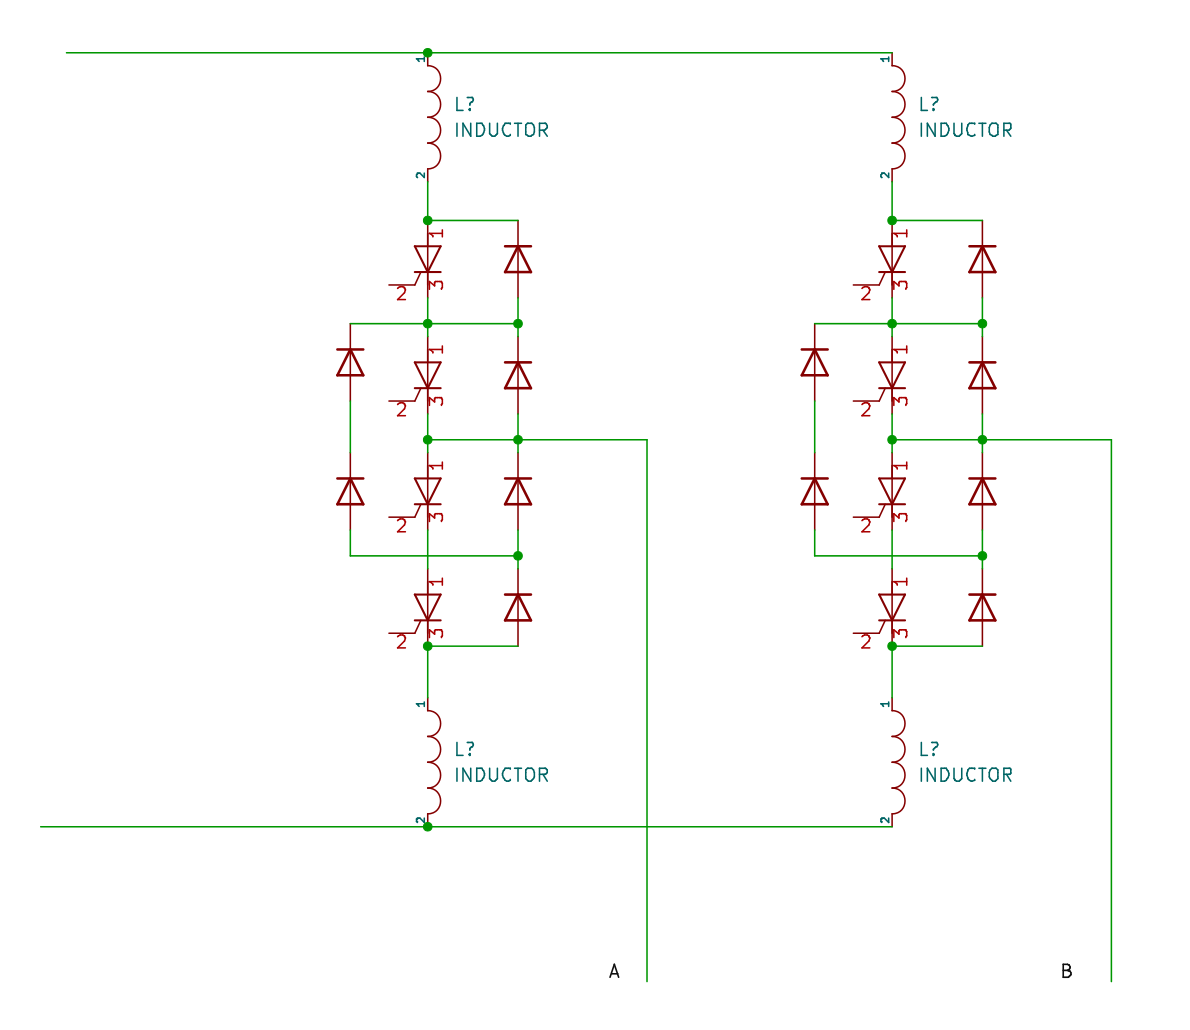
\includegraphics[width=\textwidth/2,frame]{Bilder/umrichter_schaltbild.png}
\end{figure}
\subsection{Bemessungsdaten Umrichter}
\begin{table}[htb]
    \centering
    \begin{NiceTabular}{|l|p{2cm}|}[hvlines]
        \CodeBefore
        \columncolor{lightergray}{1}
        \Body
         Nennleistung  & $\SI{5}{\unit{\mega\volt\ampere}}$\\
         Nenneingangsspannung DC  & $\SI{5000}{\V}$\\
         Nennausgangaspannung AC (RMS) & $\SI{3535}{\V}$\\
         Nennfrequenz AC-Seite  & $\SI{16.7}{\Hz}$\\
         Wirkungsgrad& $>95\%$\\    
         max. Strombelastung Halbleiter & \SI[]{1714}[]{\A}\\ 
         max. Spannungsbelastung Halbleiter & \SI[]{2500}[]{\V}\\
    \end{NiceTabular}
\end{table}

\subsubsection*{Kühlung}
Die Wechselrichter werden über ein autake Wasserkühlung gekühhlt. Pumpen befördern das Kühlwasser von den Halbleitern 
zum Wärmetauscher. Über diesen Wärmetauscher werden die Verluste des Wechselrichters an die Umgebung abgegeben. 

\subsection{Funktionsprüfung}

\begin{itemize}
    \item Spannungsprüfungen nach Isolationskoordinaten 
    \item 
\end{itemize}
                                                            \clearpage
%\section{Berechnungen}

\textbf{Nennleistung ohne Leistung der Filterwicklung:}
\begin{equation}
    S_\mathrm{N}=\frac{P_\mathrm{N}}{cos \Phi_\mathrm{max}}=\frac{\SI{16}{\MW}}{0.8}=\SI{20}{\mega\voltampere} 
\end{equation} \clearpage

\newacronym{4QS}{4QS}{Vierquadrantensteller}
%Anhang
\pagenumbering{Alph}

%Abbildungsverzeichnis
%\listoffigures \clearpage
%Tabellenverzeichnis
%\listoftables \clearpage
%Quelltextverzeichnis
%\lstlistoflistings \clearpage
%Stichwortverzeichnis
%\printindex \clearpage
%Glossar
%\printglossary[title={Glossar}] \clearpage
%Abkürzungsverzeichnis
%\printglossary[style=dottedlocations,type=\acronymtype,title={Abkürzungsverzeichnis}] \clearpage

%Literaturverzeichnisse (getrennt nach Stichwort)
%\printbibliography[heading=bibintoc, keyword={book}, %title={Literaturverzeichnis}]\clearpage
%\printbibliography[heading=bibintoc, keyword={online}, title={Onlinequellen}]\clearpage
%\printbibliography[heading=bibintoc, keyword={image}, title={Bildquellen}]\clearpage
\printbibliography[title={Normative Verweise}]\clearpage
% Anhang
\appendix
\section{Anhang}
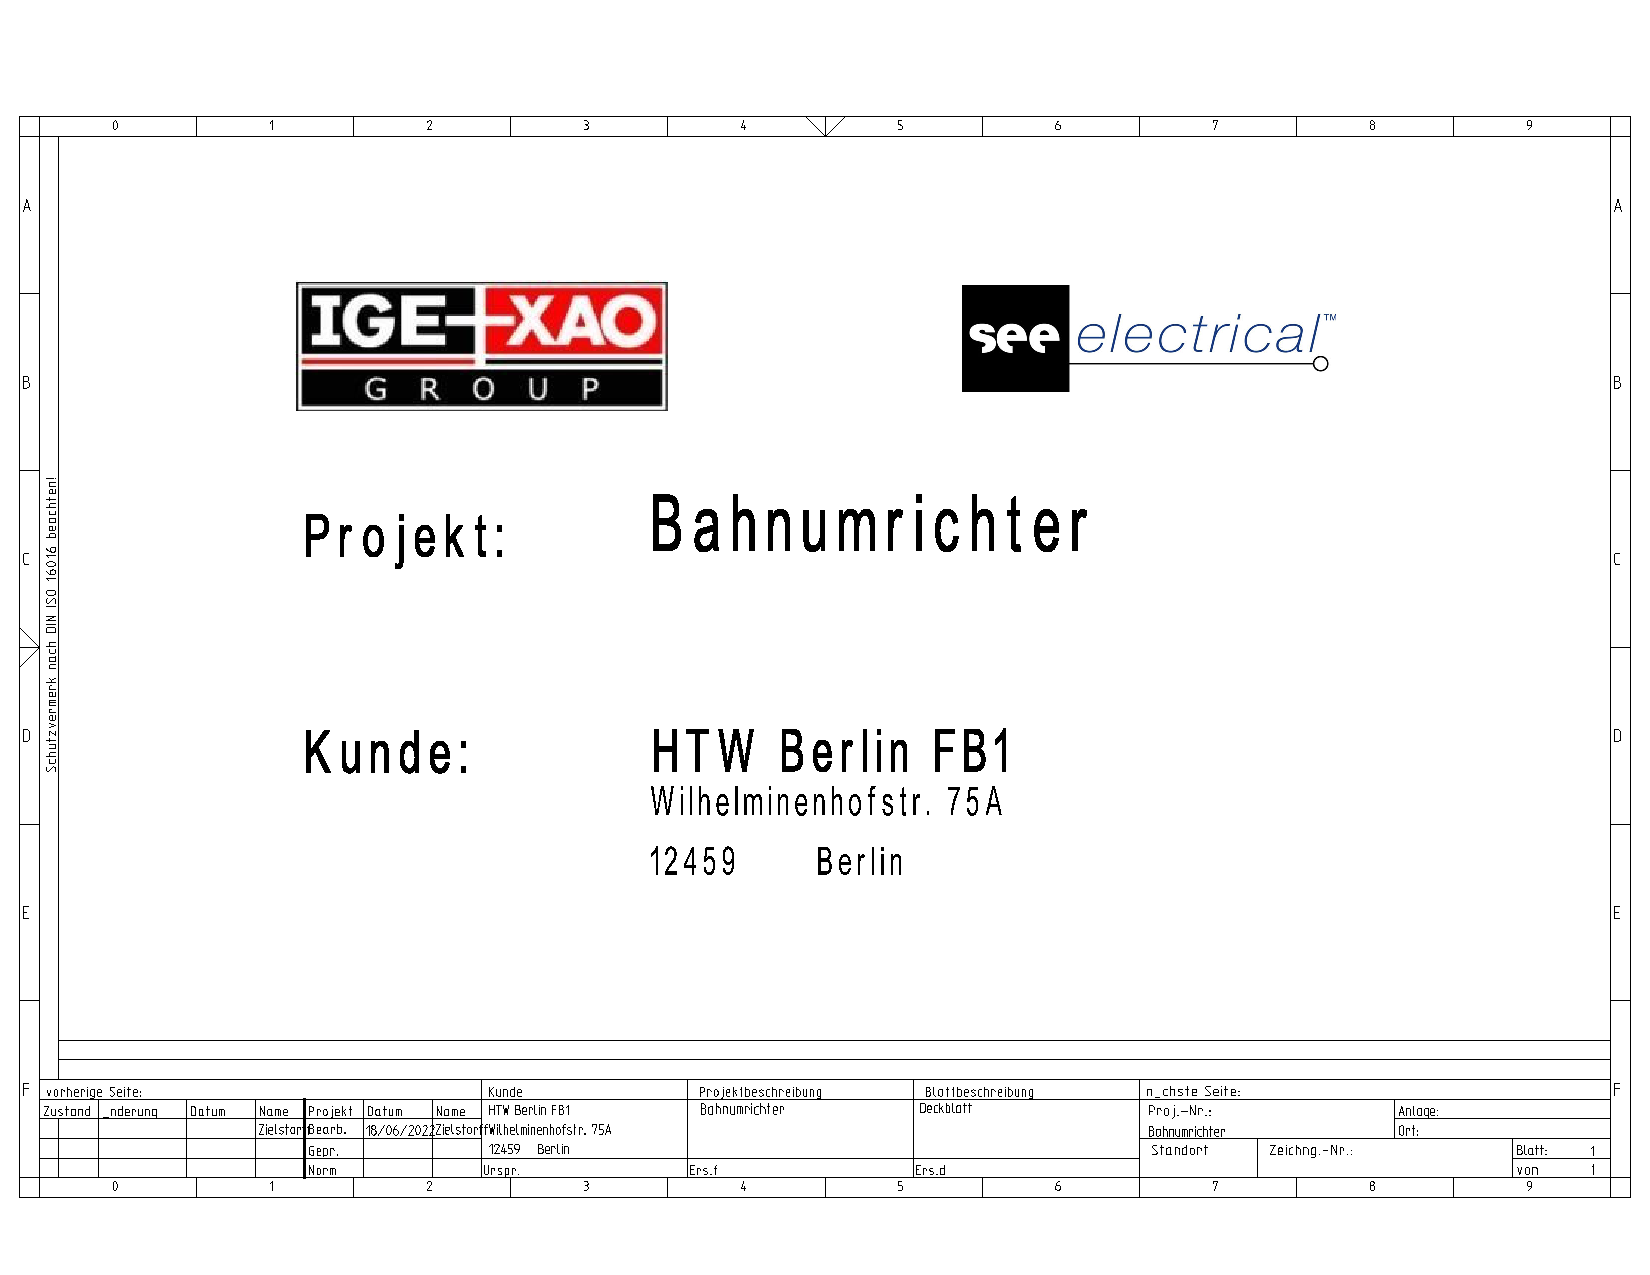
\includepdf[pages=-,landscape]{Bilder/cad.pdf}



% Eigenständigkeitserklärung
%\input{chapter/Eigenstaendigkeitserklaerung}
\end{document}